\def\secforfig{appendices/bkgd-mc-validation}
\def\figsversion{V1}

\begin{figure}[ht]
    \centering
    \subfloat[${\pt}_{2}$]{%
            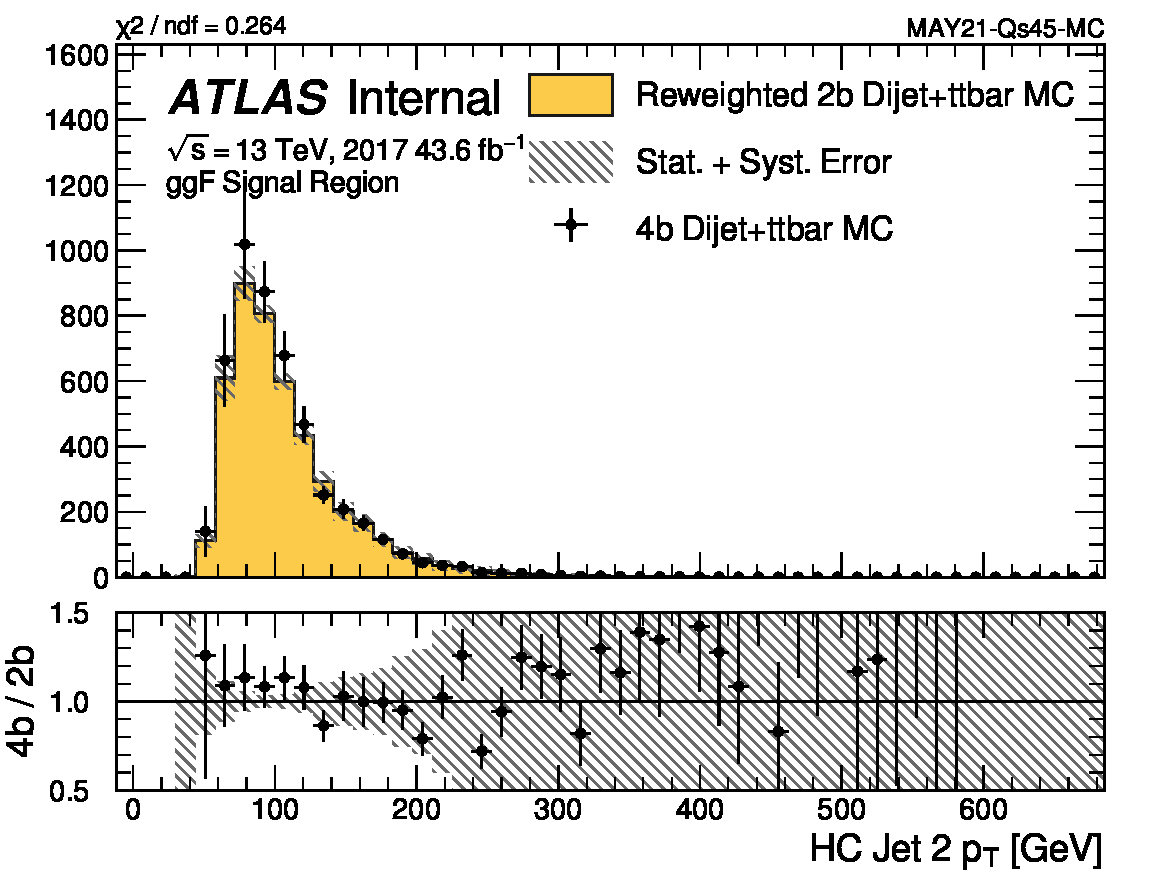
\includegraphics[width=0.25\textwidth]{\figpath{data-weights/bkgd-4b-nocat/sig/2017/MAY21-Qs45-MC-pT-2-Signal-NN-17-4binclusive.pdf}}
    }
    \subfloat[${\pt}_{4}$]{%
            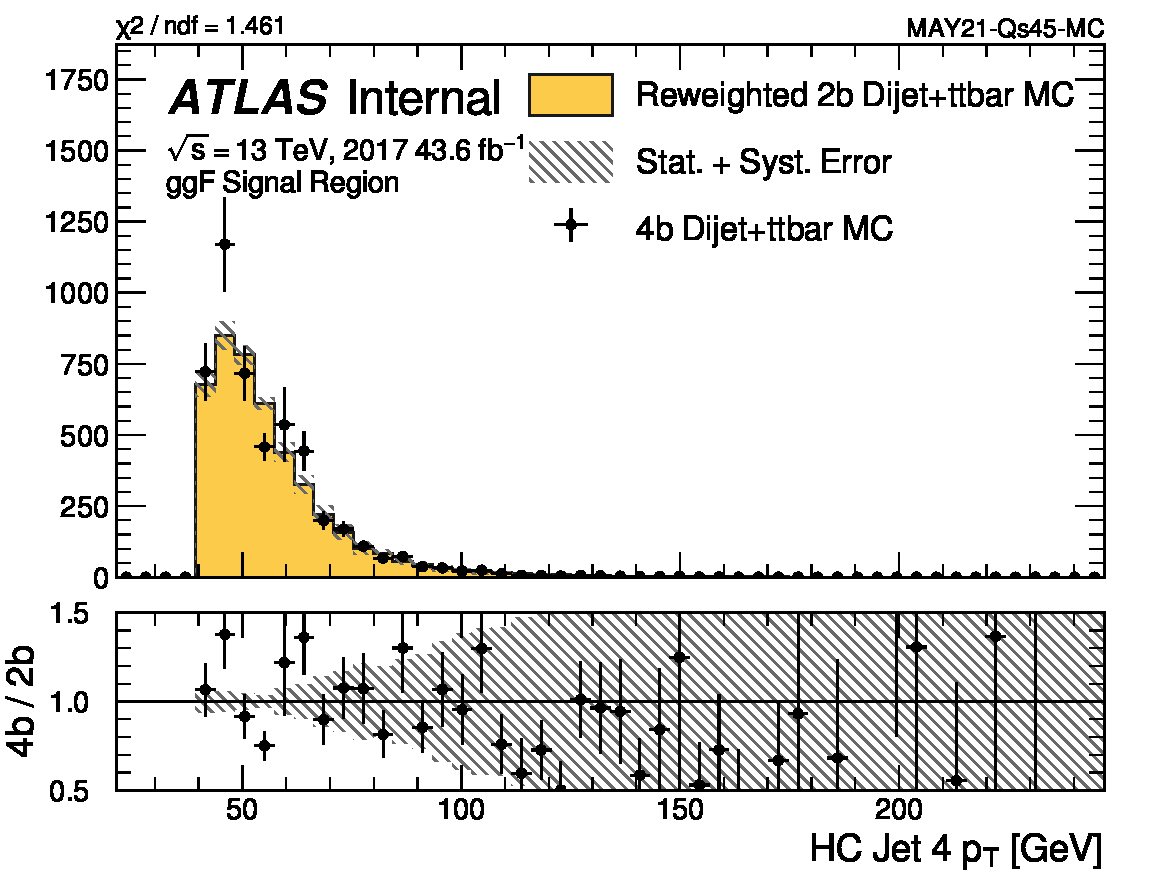
\includegraphics[width=0.25\textwidth]{\figpath{data-weights/bkgd-4b-nocat/sig/2017/MAY21-Qs45-MC-pT-4-Signal-NN-17-4binclusive.pdf}}
    }
    \subfloat[$dR_{jj,1}$]{%
            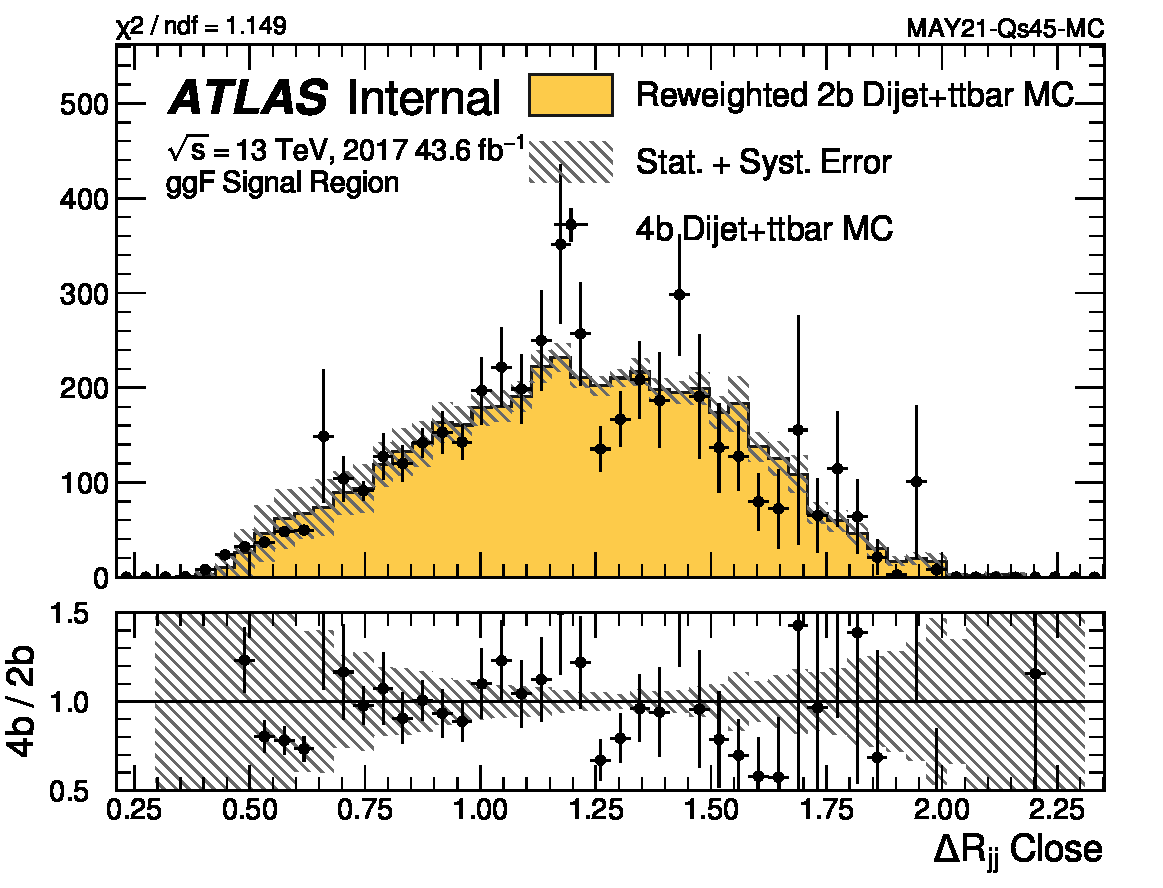
\includegraphics[width=0.25\textwidth]{\figpath{data-weights/bkgd-4b-nocat/sig/2017/MAY21-Qs45-MC-dRjj-1-Signal-NN-17-4binclusive.pdf}}
    }
    \subfloat[$dR_{jj,2}$]{%
            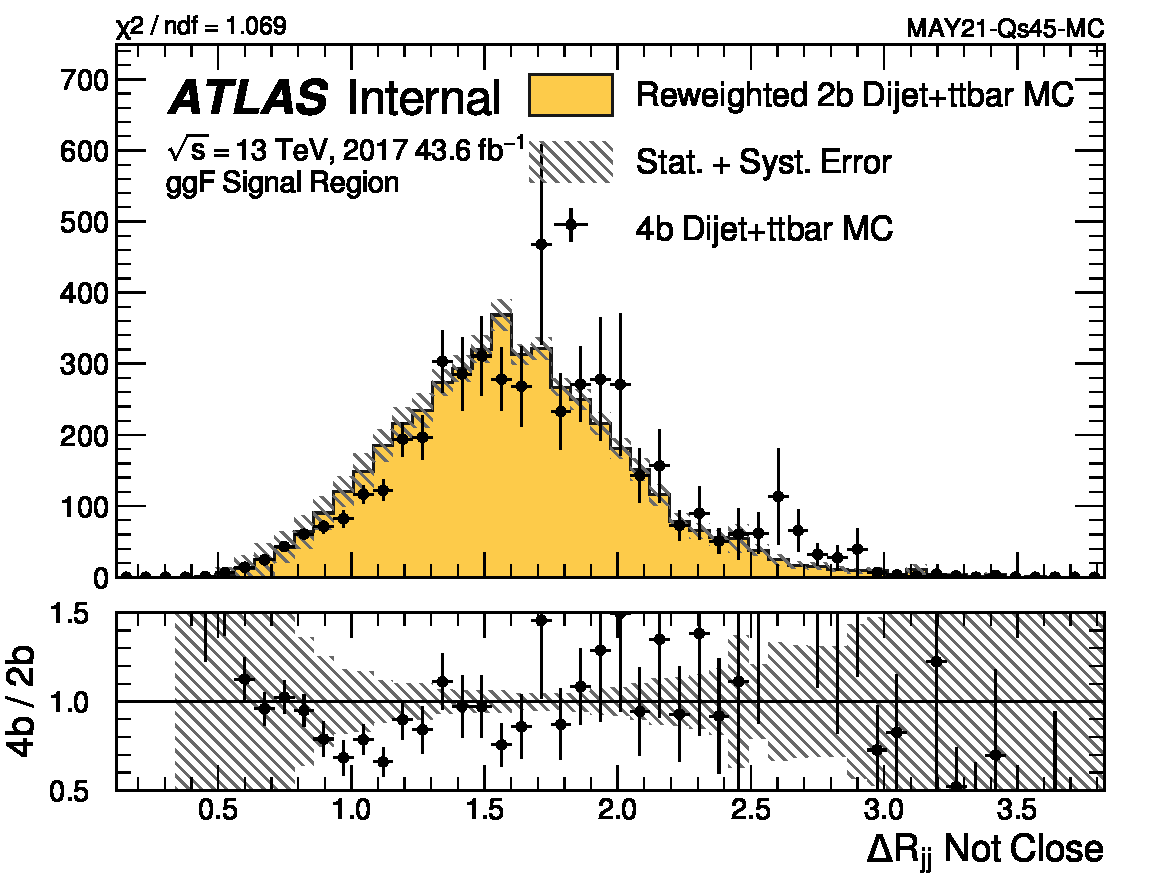
\includegraphics[width=0.25\textwidth]{\figpath{data-weights/bkgd-4b-nocat/sig/2017/MAY21-Qs45-MC-dRjj-2-Signal-NN-17-4binclusive.pdf}}
    }

    \subfloat[$\eta_{i}$]{%
            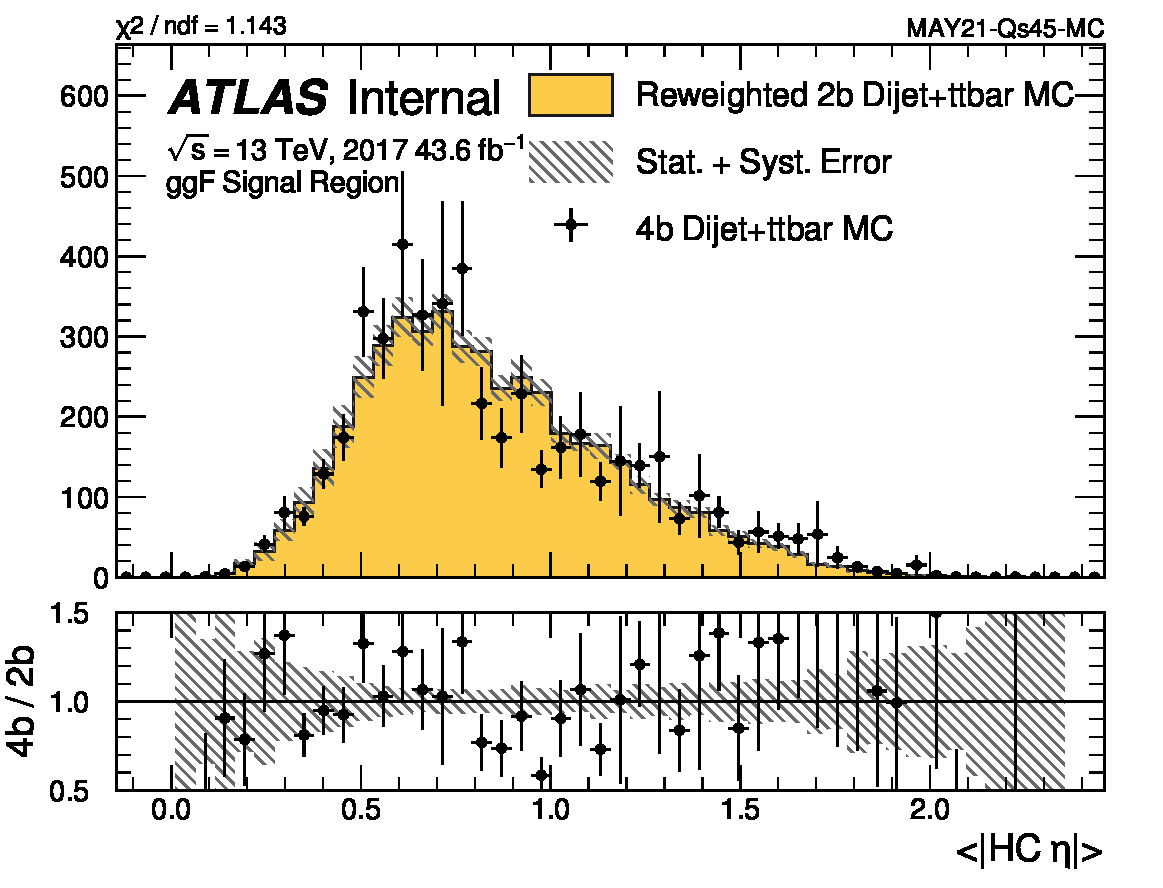
\includegraphics[width=0.25\textwidth]{\figpath{data-weights/bkgd-4b-nocat/sig/2017/MAY21-Qs45-MC-eta-i-Signal-NN-17-4binclusive.pdf}}
    }
    \subfloat[${\pt}_{\higgs\higgs}$]{%
            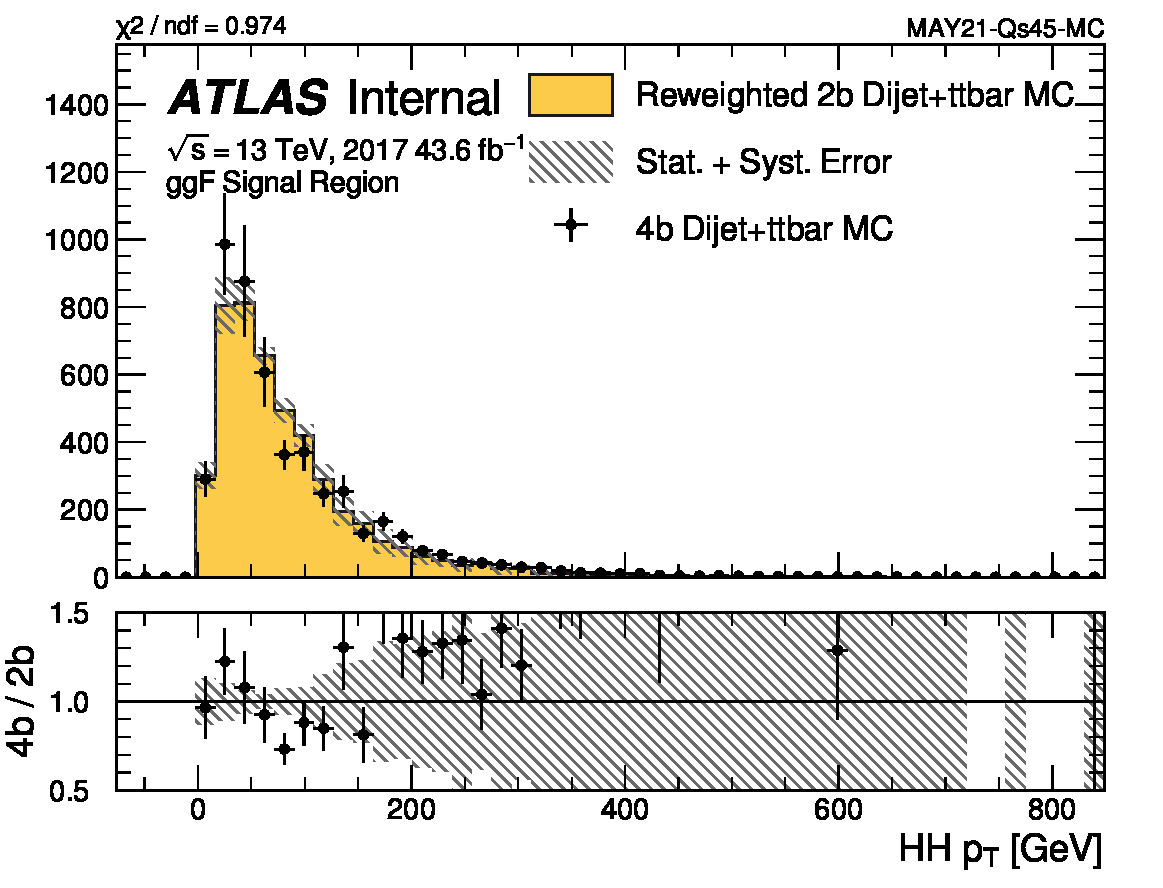
\includegraphics[width=0.25\textwidth]{\figpath{data-weights/bkgd-4b-nocat/sig/2017/MAY21-Qs45-MC-pt-hh-Signal-NN-17-4binclusive.pdf}}
    }
    \subfloat[$dPhi_{\PH1}$]{%
            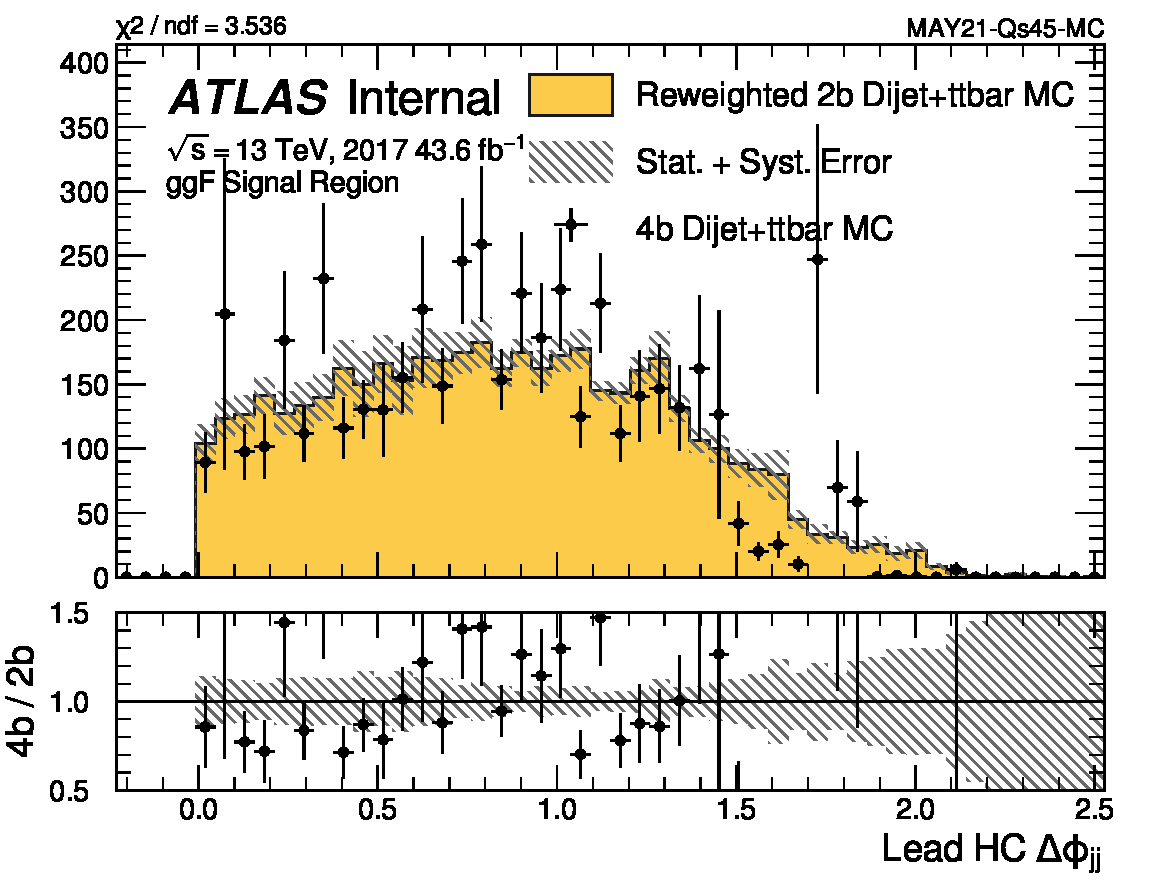
\includegraphics[width=0.25\textwidth]{\figpath{data-weights/bkgd-4b-nocat/sig/2017/MAY21-Qs45-MC-dPhi-h1-Signal-NN-17-4binclusive.pdf}}
    }
    \subfloat[$dPhi_{\PH2}$]{%
            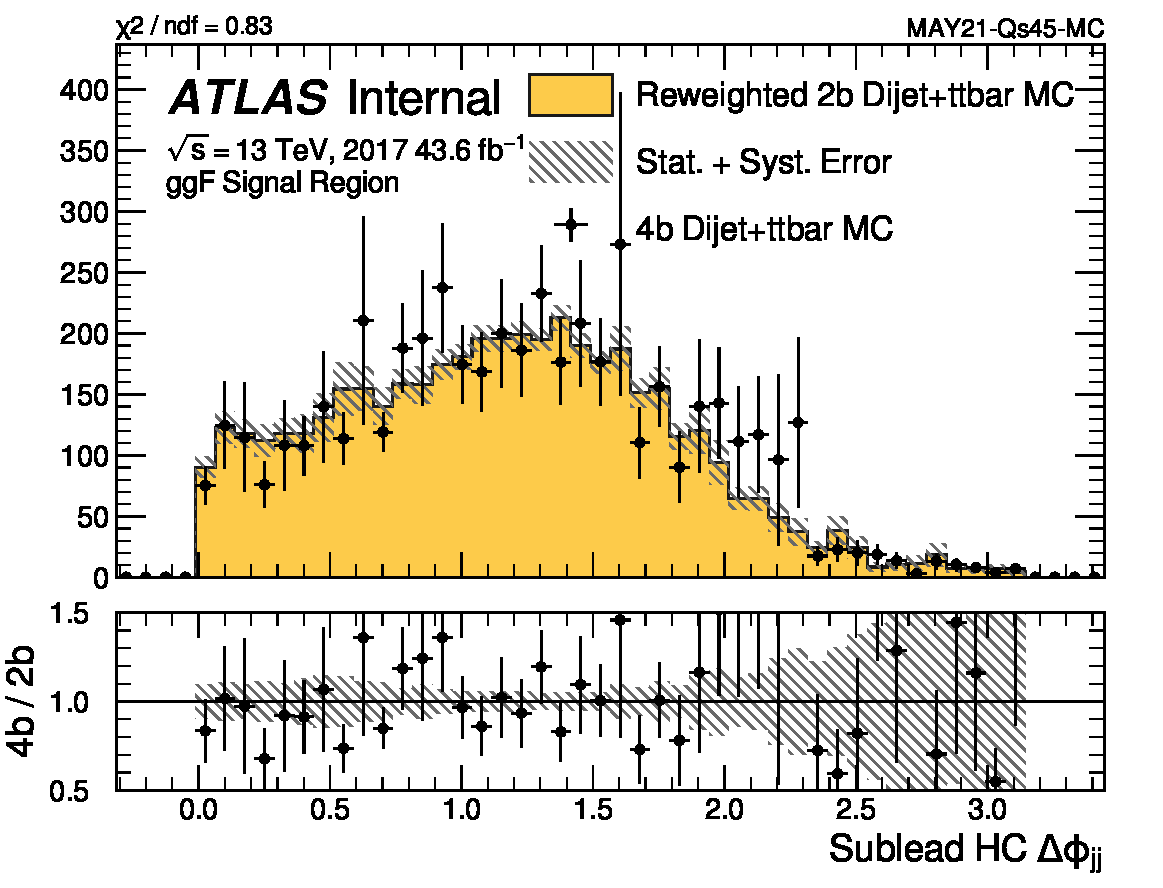
\includegraphics[width=0.25\textwidth]{\figpath{data-weights/bkgd-4b-nocat/sig/2017/MAY21-Qs45-MC-dPhi-h2-Signal-NN-17-4binclusive.pdf}}
    }

    \subfloat[$dR_{\higgs\higgs}$]{%
            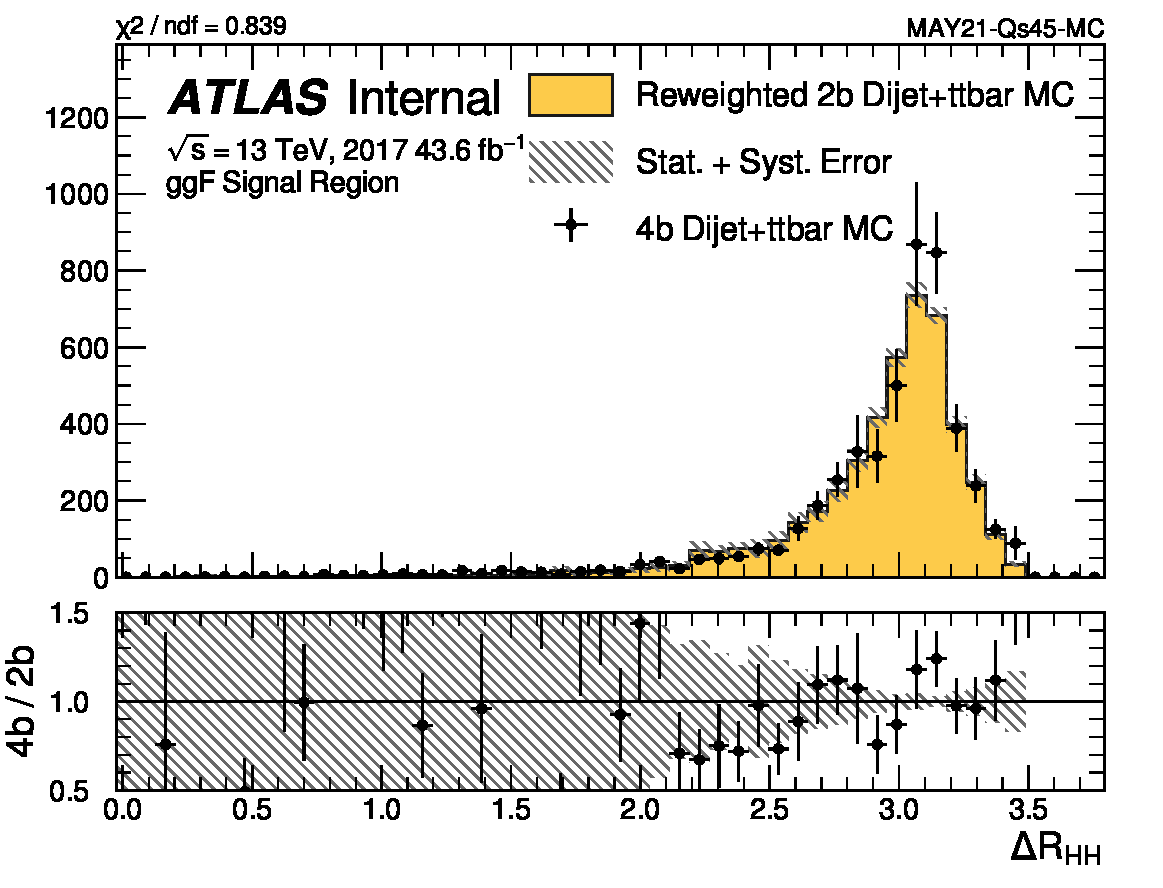
\includegraphics[width=0.25\textwidth]{\figpath{data-weights/bkgd-4b-nocat/sig/2017/MAY21-Qs45-MC-dR-hh-Signal-NN-17-4binclusive.pdf}}
    }
    \subfloat[$dEta_{\higgs\higgs}$]{%
            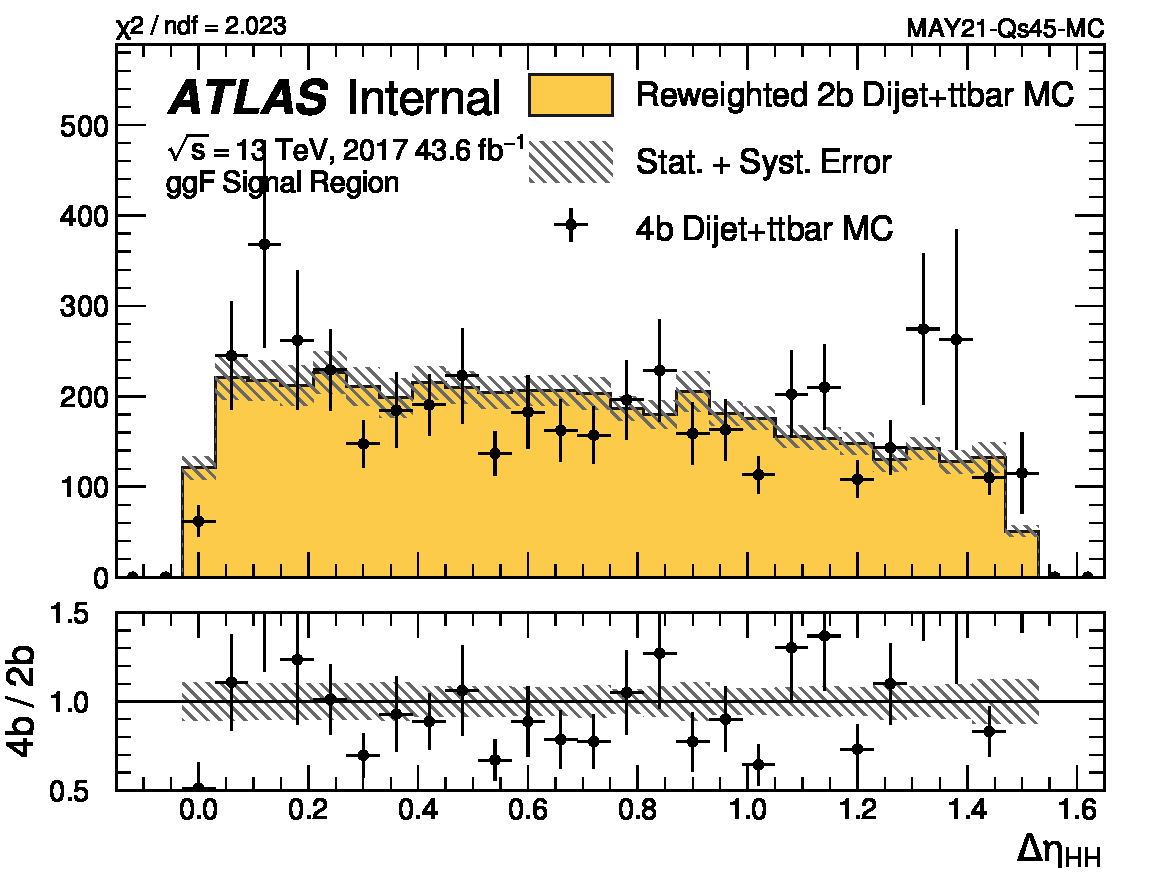
\includegraphics[width=0.25\textwidth]{\figpath{data-weights/bkgd-4b-nocat/sig/2017/MAY21-Qs45-MC-dEta-hh-Signal-NN-17-4binclusive.pdf}}
    }
    \subfloat[$X_{wt}$]{%
            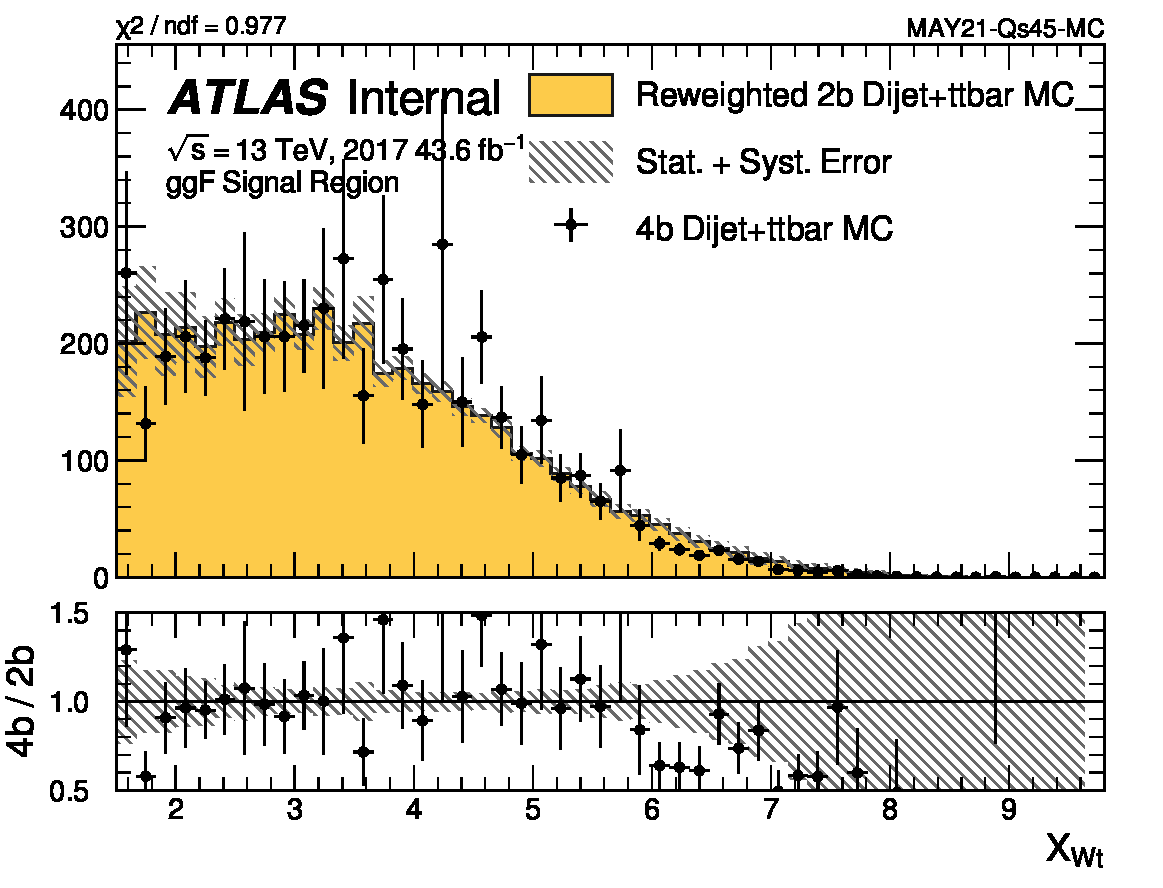
\includegraphics[width=0.25\textwidth]{\figpath{data-weights/bkgd-4b-nocat/sig/2017/MAY21-Qs45-MC-X-wt-tag-Signal-NN-17-4binclusive.pdf}}
    }
    \subfloat[njets]{%
            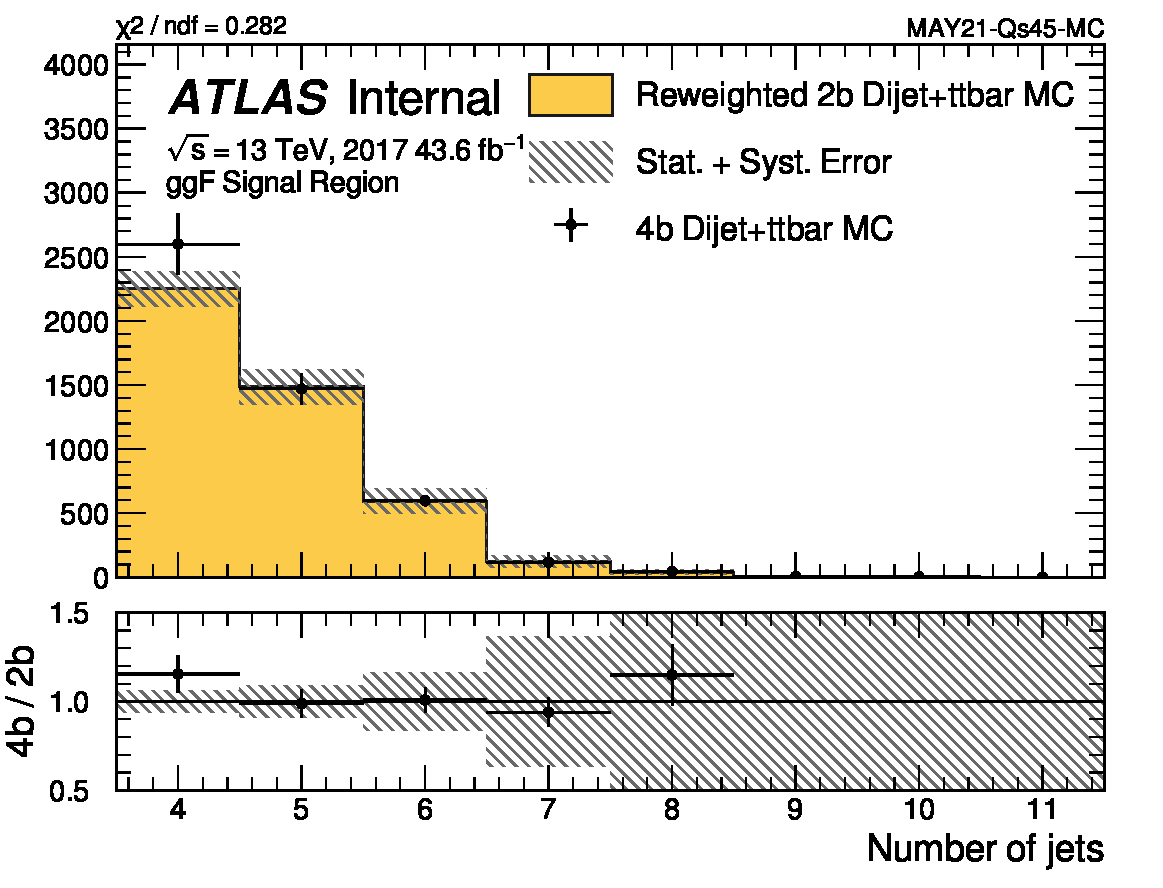
\includegraphics[width=0.25\textwidth]{\figpath{data-weights/bkgd-4b-nocat/sig/2017/MAY21-Qs45-MC-njets-Signal-NN-17-4binclusive.pdf}}
    }

    \subfloat[${\pt}_{\PH1}$]{%
            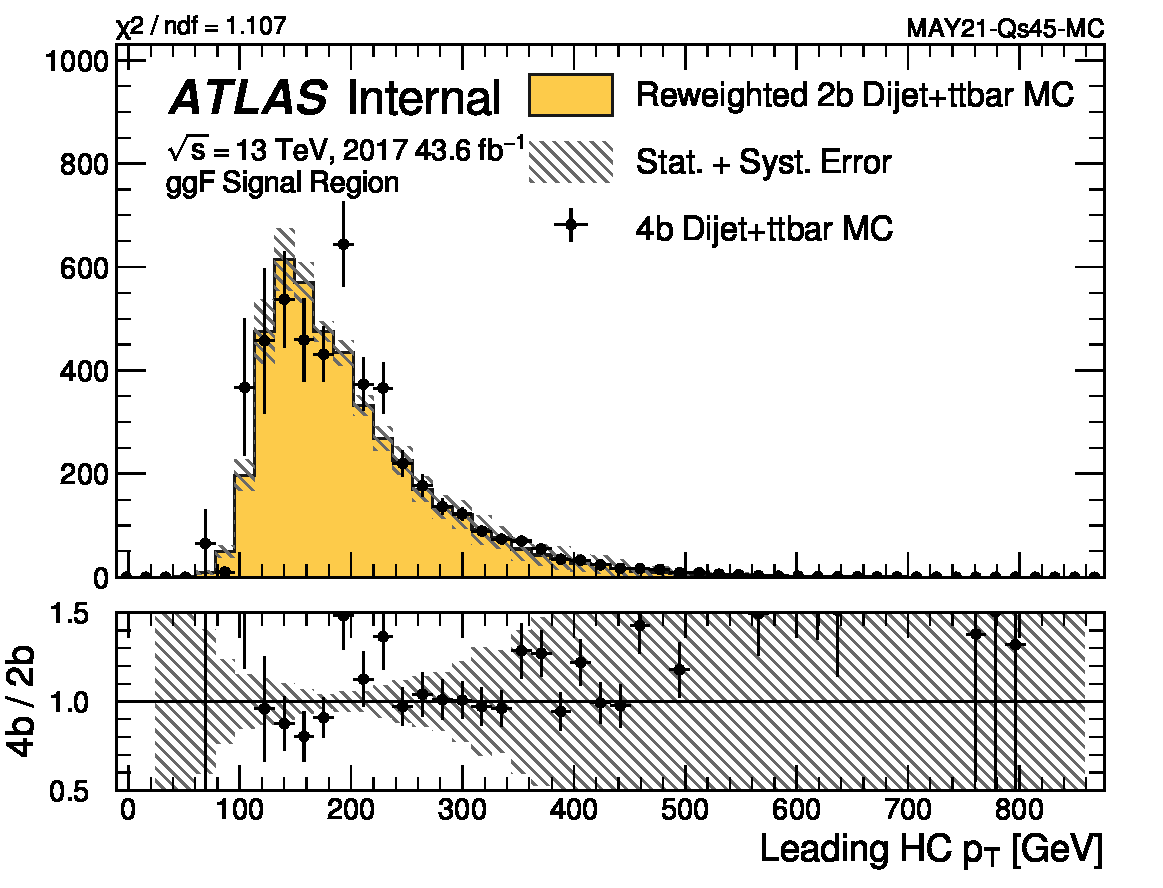
\includegraphics[width=0.25\textwidth]{\figpath{data-weights/bkgd-4b-nocat/sig/2017/MAY21-Qs45-MC-pT-h1-Signal-NN-17-4binclusive.pdf}}
    }
    \subfloat[${\pt}_{\PH2}$]{%
            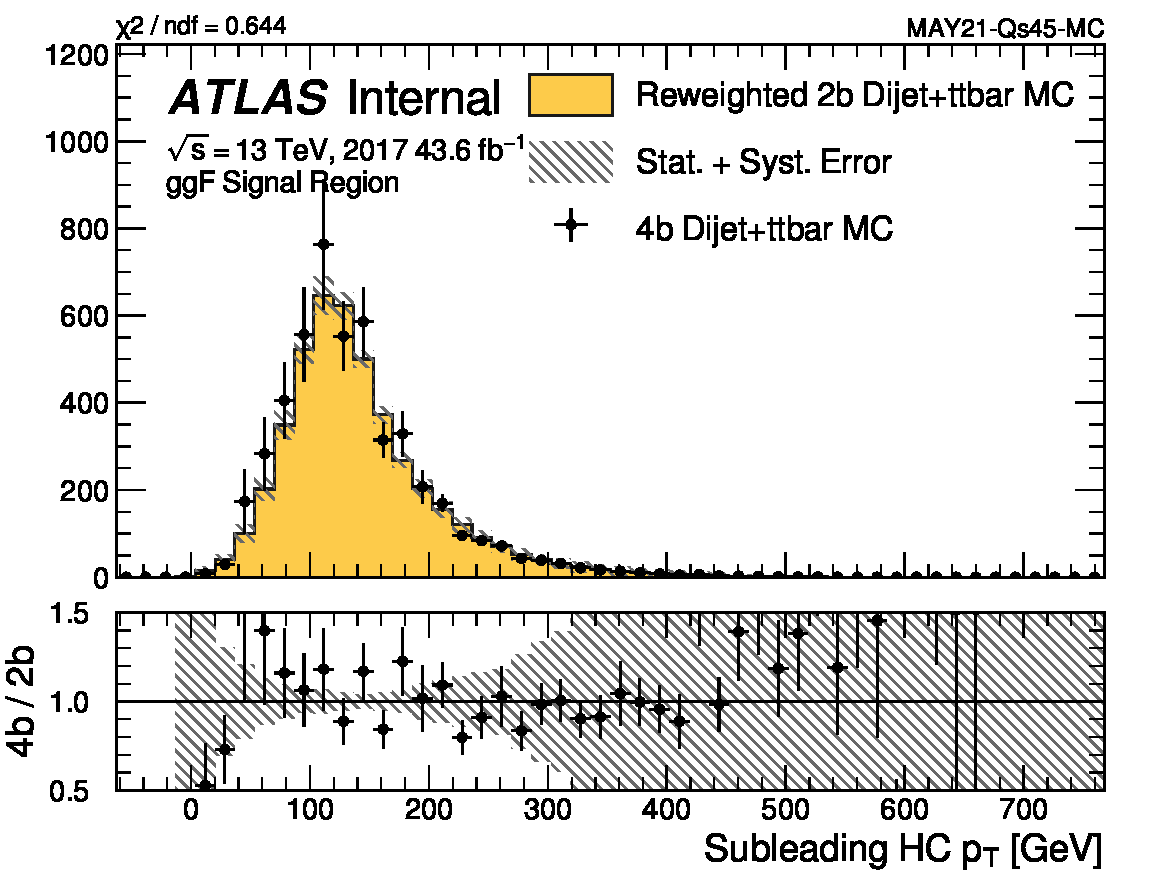
\includegraphics[width=0.25\textwidth]{\figpath{data-weights/bkgd-4b-nocat/sig/2017/MAY21-Qs45-MC-pT-h2-Signal-NN-17-4binclusive.pdf}}
    }
    \subfloat[$m_{\PH1}$]{%
            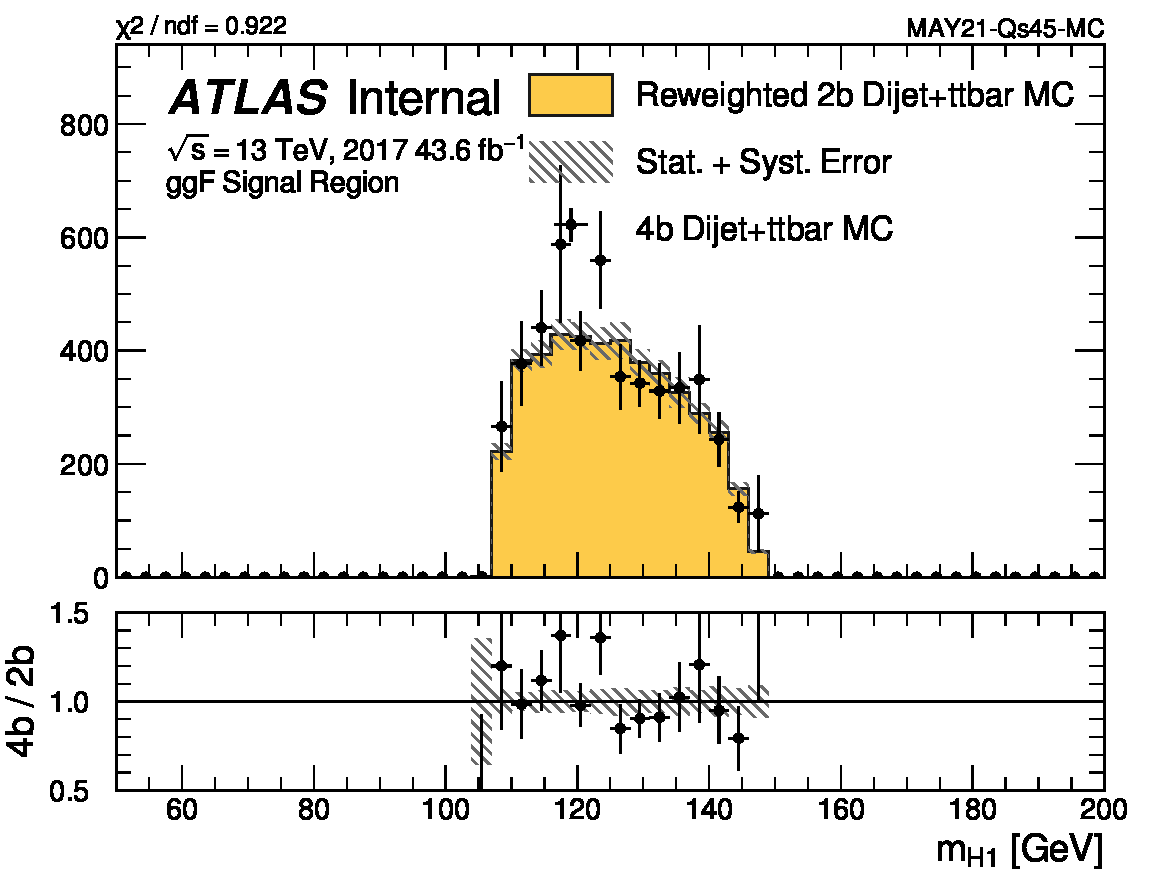
\includegraphics[width=0.25\textwidth]{\figpath{data-weights/bkgd-4b-nocat/sig/2017/MAY21-Qs45-MC-m-h1-Signal-NN-17-4binclusive.pdf}}
    }
    \subfloat[$m_{\PH2}$]{%
            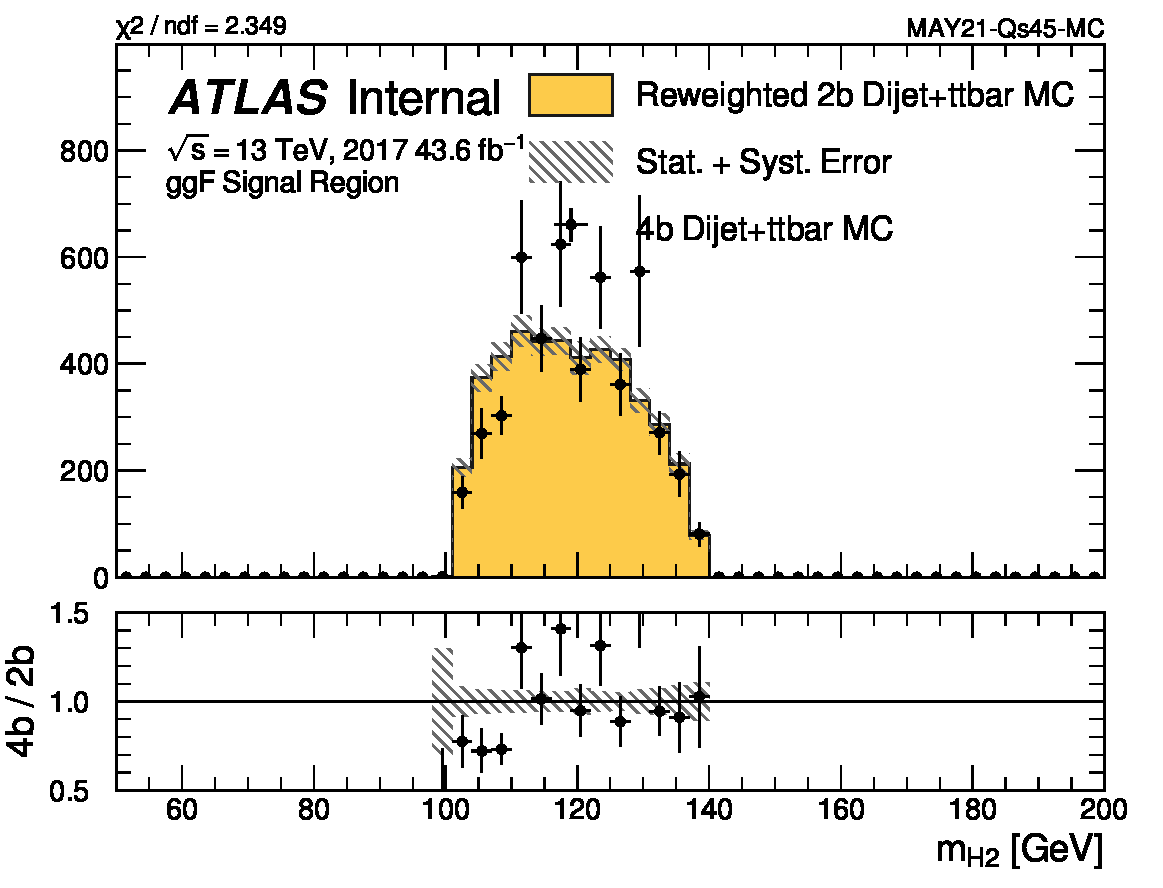
\includegraphics[width=0.25\textwidth]{\figpath{data-weights/bkgd-4b-nocat/sig/2017/MAY21-Qs45-MC-m-h2-Signal-NN-17-4binclusive.pdf}}
    }

    %%%\subfloat[$\eta_{1}$]{%
    %%%        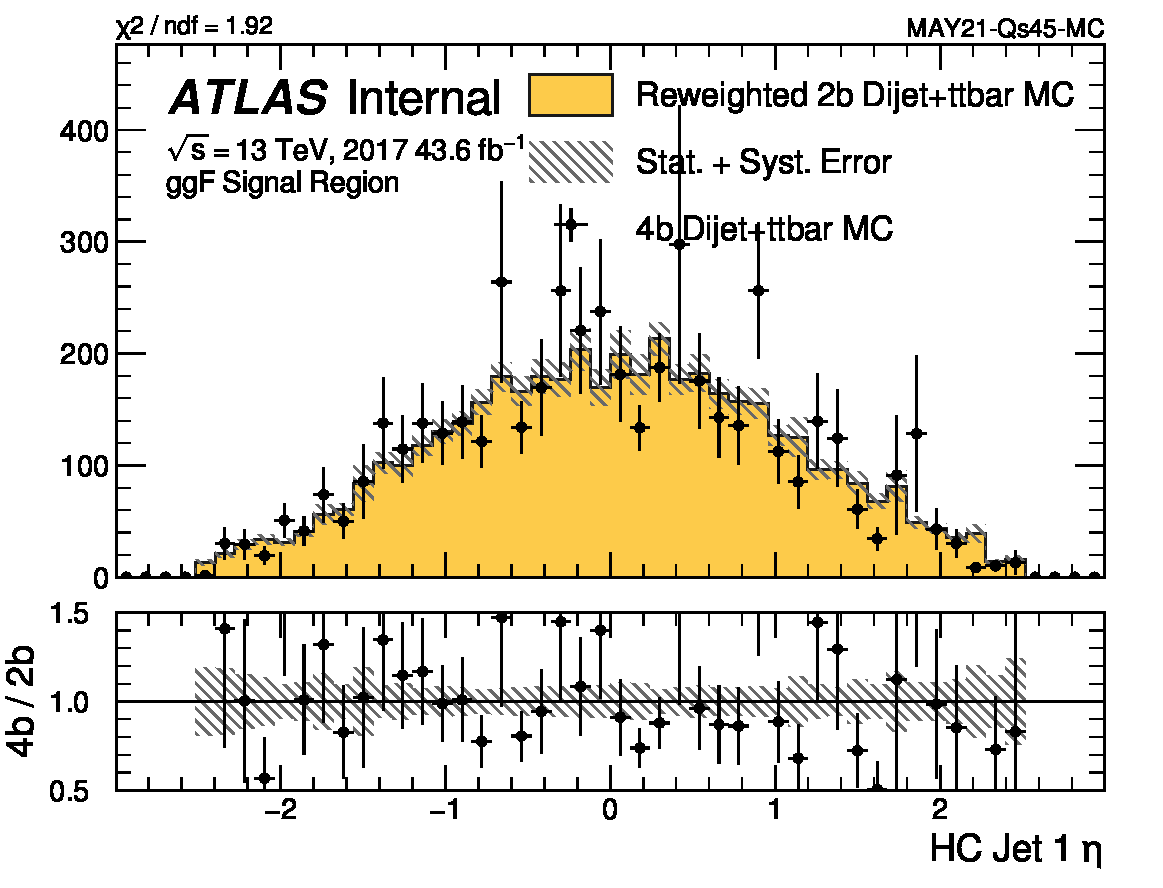
\includegraphics[width=0.25\textwidth]{\figpath{data-weights/bkgd-4b-nocat/sig/2017/MAY21-Qs45-MC-eta-1-Signal-NN-17-4binclusive.pdf}}
    %%%}
    %%%\subfloat[$\eta_{2}$]{%
    %%%        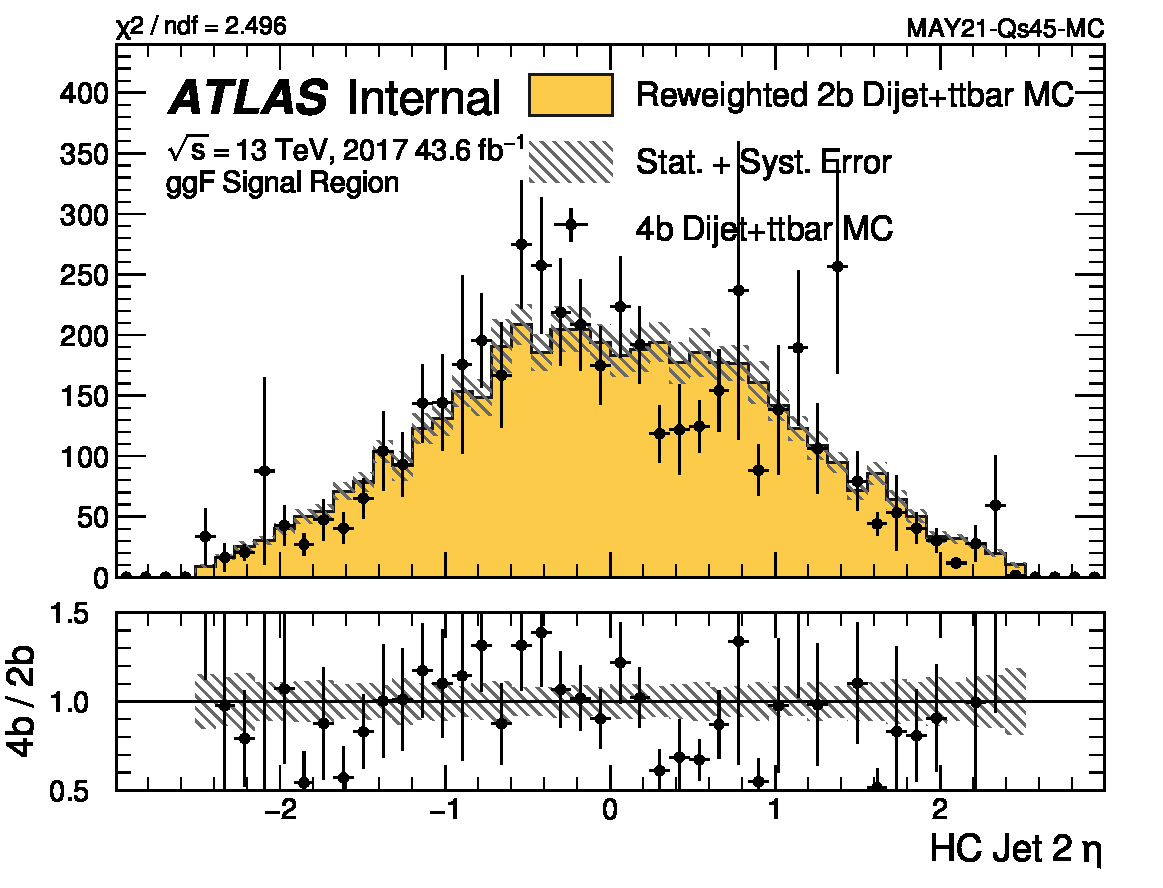
\includegraphics[width=0.25\textwidth]{\figpath{data-weights/bkgd-4b-nocat/sig/2017/MAY21-Qs45-MC-eta-2-Signal-NN-17-4binclusive.pdf}}
    %%%}
    %%%\subfloat[$\eta_{3}$]{%
    %%%        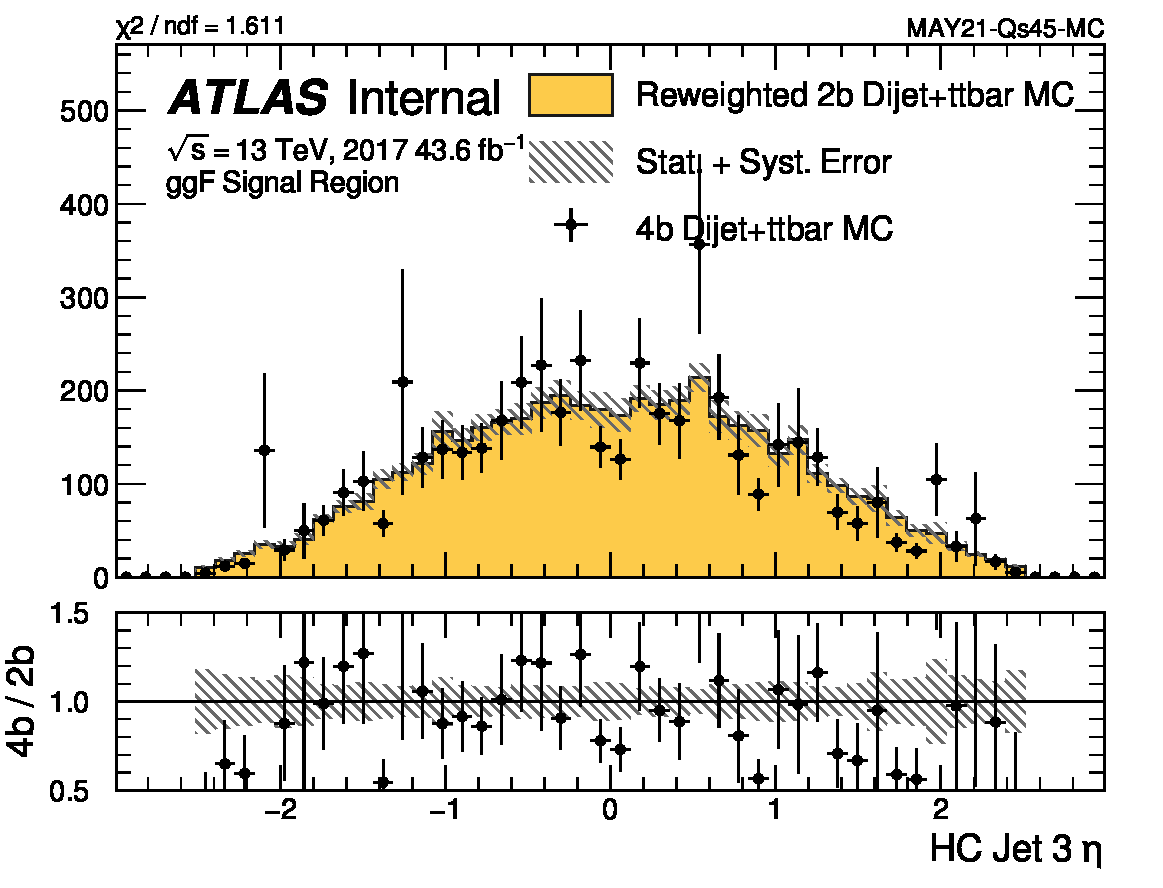
\includegraphics[width=0.25\textwidth]{\figpath{data-weights/bkgd-4b-nocat/sig/2017/MAY21-Qs45-MC-eta-3-Signal-NN-17-4binclusive.pdf}}
    %%%}
    %%%\subfloat[$\eta_{4}$]{%
    %%%        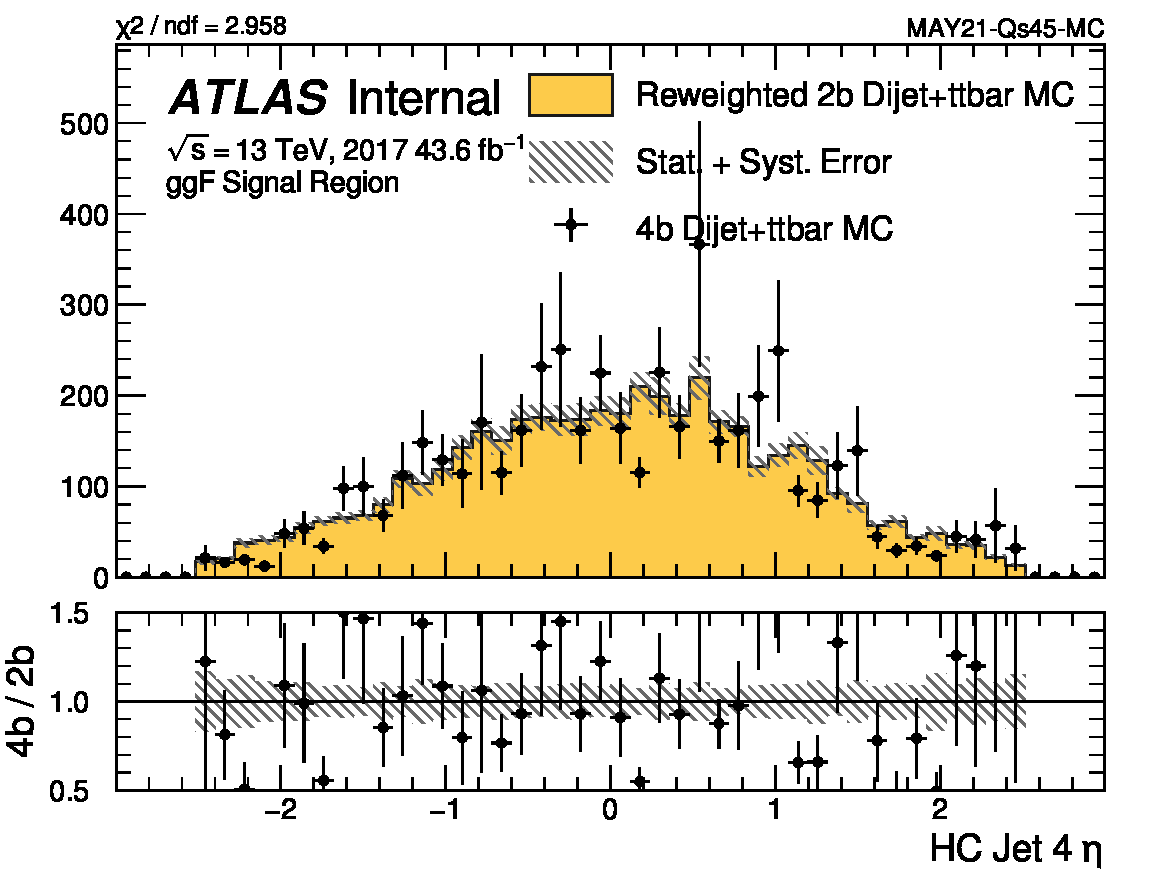
\includegraphics[width=0.25\textwidth]{\figpath{data-weights/bkgd-4b-nocat/sig/2017/MAY21-Qs45-MC-eta-4-Signal-NN-17-4binclusive.pdf}}
    %%%}
 
    %%%\subfloat[${\pt}_{1}$]{%
    %%%        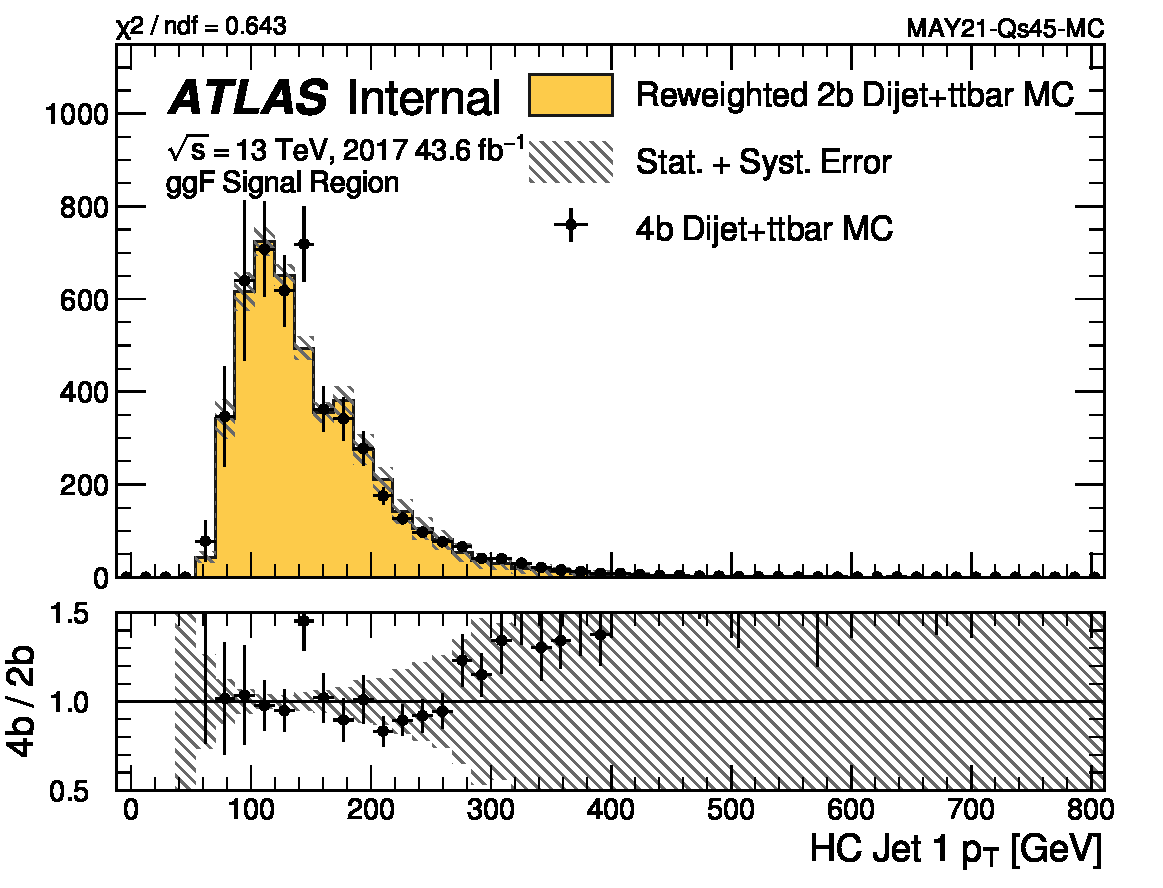
\includegraphics[width=0.25\textwidth]{\figpath{data-weights/bkgd-4b-nocat/sig/2017/MAY21-Qs45-MC-pT-1-Signal-NN-17-4binclusive.pdf}}
    %%%}
    %%%\subfloat[${\pt}_{2}$]{%
    %%%        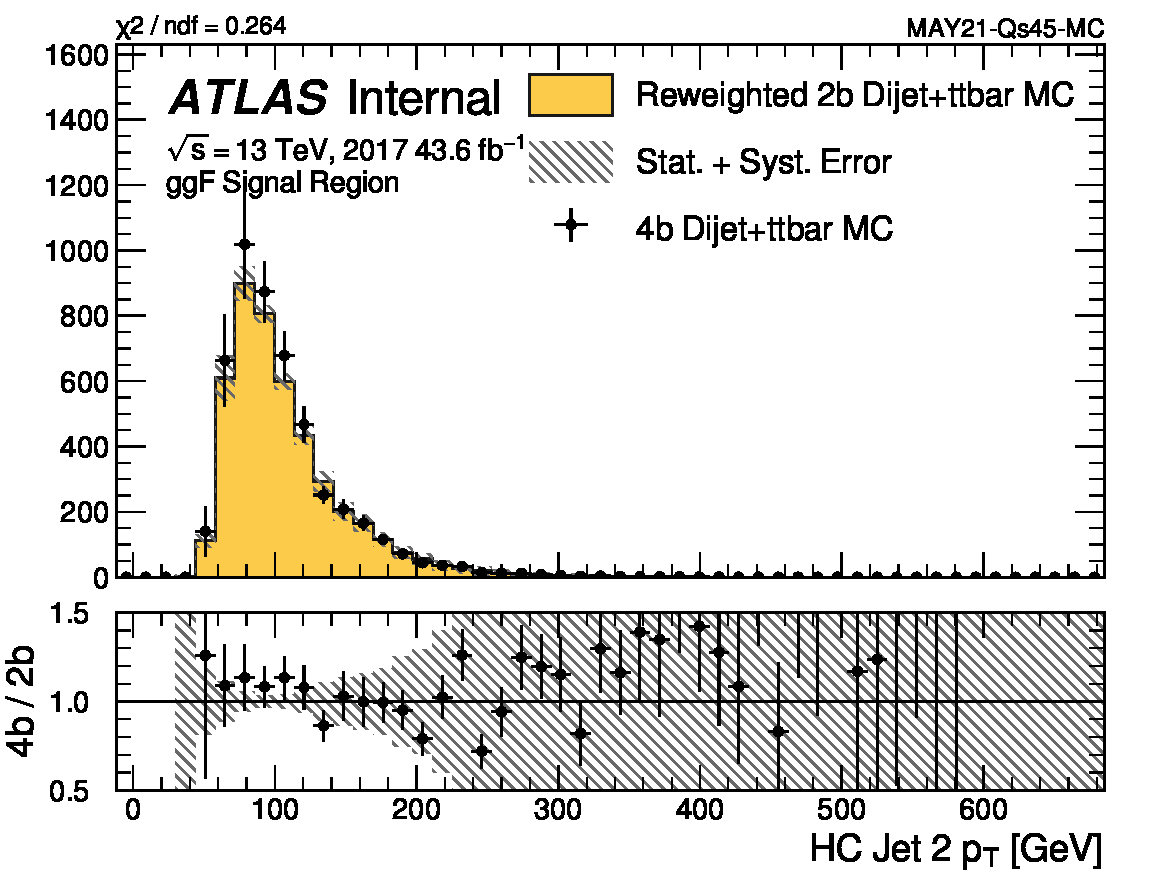
\includegraphics[width=0.25\textwidth]{\figpath{data-weights/bkgd-4b-nocat/sig/2017/MAY21-Qs45-MC-pT-2-Signal-NN-17-4binclusive.pdf}}
    %%%}
    %%%\subfloat[${\pt}_{3}$]{%
    %%%        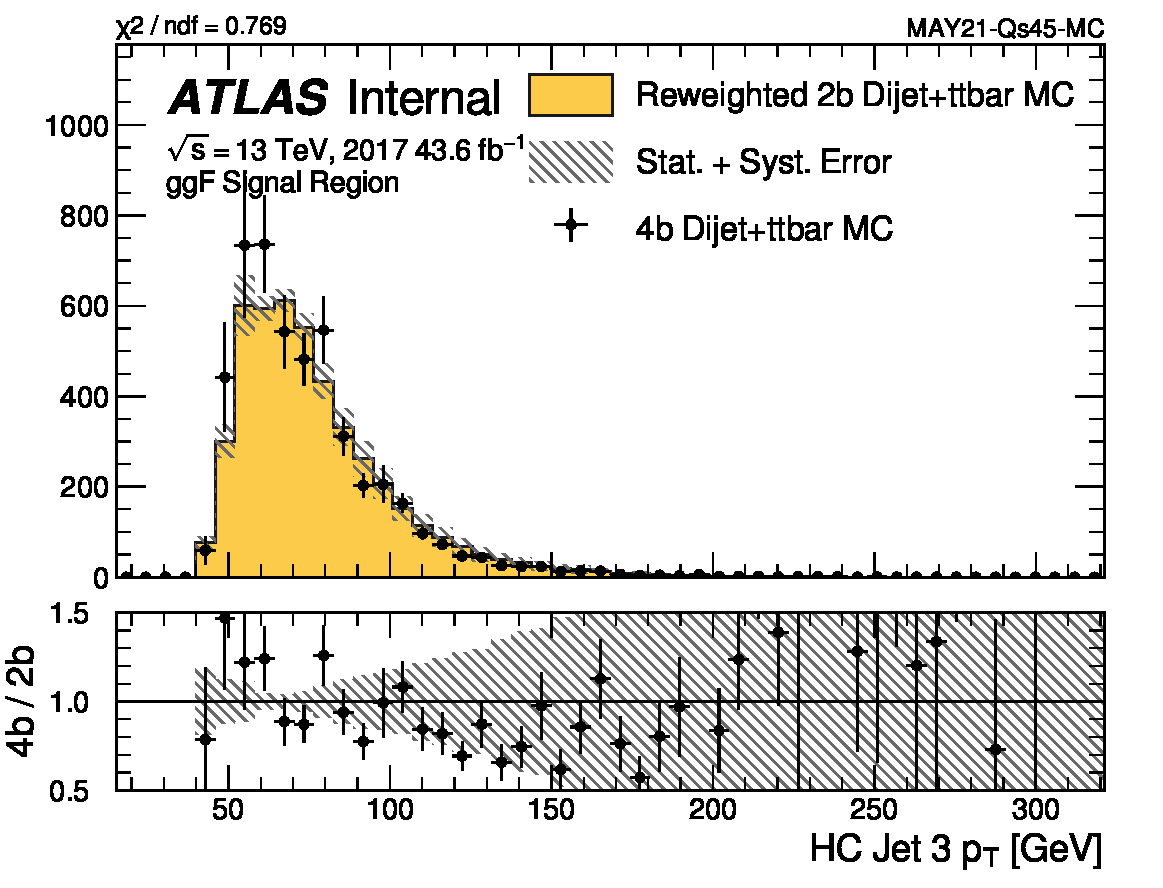
\includegraphics[width=0.25\textwidth]{\figpath{data-weights/bkgd-4b-nocat/sig/2017/MAY21-Qs45-MC-pT-3-Signal-NN-17-4binclusive.pdf}}
    %%%}
    %%%\subfloat[${\pt}_{4}$]{%
    %%%        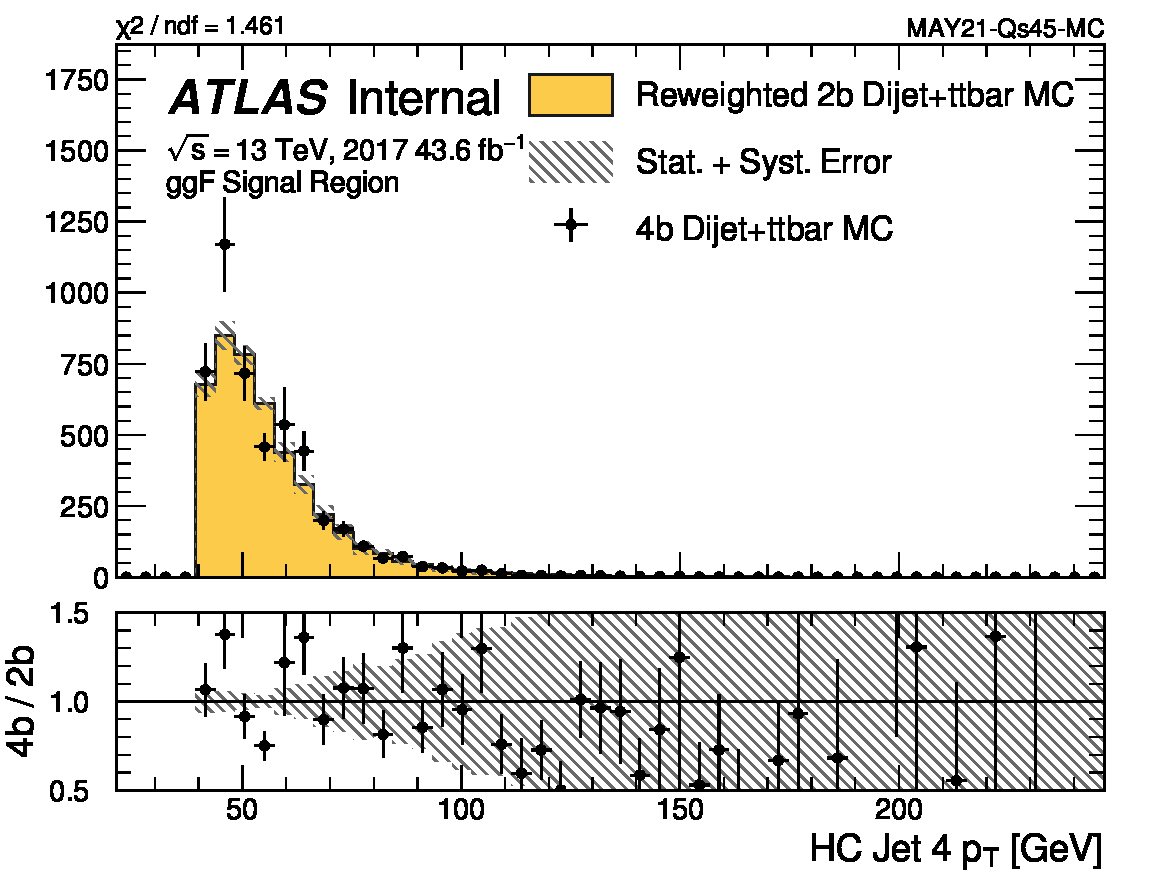
\includegraphics[width=0.25\textwidth]{\figpath{data-weights/bkgd-4b-nocat/sig/2017/MAY21-Qs45-MC-pT-4-Signal-NN-17-4binclusive.pdf}}
    %%%}

    \caption{4b and reweighted 2b distributions of QCD and \ttbar MC samples in Signal Region in 2017.}
    \label{fig:data-weights-4b-SR-2017}
\end{figure}


